\documentclass[a4paper]{article}

%deixa no padr?o brasileiro, traduzindo as se??es, possibilitando caracteres e hifen
\usepackage[brazilian]{babel}
\usepackage[utf8]{inputenc}
\usepackage[T1]{fontenc}
\usepackage{amsmath,amsthm,array} 

%estilo de header
\pagestyle{headings}

%pacote para inserir imagem
\usepackage{graphicx}

\usepackage{listings}
\usepackage{color}
\definecolor{lightgray}{rgb}{.9,.9,.9}
\definecolor{darkgray}{rgb}{.4,.4,.4}
\definecolor{purple}{rgb}{0.65, 0.12, 0.82}

\lstdefinelanguage{JavaScript}{
  keywords={typeof, new, true, false, catch, function, return, null, catch, switch, var, if, in, while, do, else, case, break},
  keywordstyle=\color{blue}\bfseries,
  ndkeywords={class, export, boolean, throw, implements, import, this},
  ndkeywordstyle=\color{darkgray}\bfseries,
  identifierstyle=\color{black},
  sensitive=false,
  comment=[l]{//},
  morecomment=[s]{/*}{*/},
  commentstyle=\color{purple}\ttfamily,
  stringstyle=\color{red}\ttfamily,
  morestring=[b]',
  morestring=[b]"
}

\lstset{
   language=JavaScript,
   backgroundcolor=\color{lightgray},
   extendedchars=true,
   basicstyle=\footnotesize\ttfamily,
   showstringspaces=false,
   showspaces=false,
   numbers=left,
   numberstyle=\footnotesize,
   numbersep=9pt,
   tabsize=2,
   breaklines=true,
   showtabs=false,
   captionpos=b
}

%t?tulo
\title{Subprogramas}
\author{Gustavo Scaloni Vendramini    \\ 
        Guilherme José Henrique       \\
        Sean Carlisto de Alvarenga    \\
        Vinícius Fernandes de Jesus}
\date{\today}

%pacote que coloca links no table of contents e monta o índice lateral, de acordo com as se??es do documento.
\usepackage[pdftex]{hyperref}

%documento em s?
\begin{document}
\maketitle
\pagebreak
\maketitle
\tableofcontents

\section{Ambiente de Referênciamento Local} 
\label{sec:ambiente_de_referenciamento_local}
Variáveis que são definidas dentro de subprogramas são chamadas de variáveis locais, porque o acesso a elas normalmente é restrito ao subprograma na qual são definidas \cite{sebesta}. Essas variáveis podem ser variáveis estáticas ou variáveis dinâmicas na pilha.

\subsection{Variáveis Locais}
\label{sub:variaveis_locais}
Variáveis estáticas são vinculadas a células de memória antes do inicio da execução do programa e continuam até o término de sua execução.Uma das vantagens de variáveis estáticas é que elas possuem um endereçamento direto na memória como mostra a figura \ref{enderecamento}, permitindo assim um acesso mais rápido em relação a variáveis com endereçamento indireto. Outra vantagem, é por não causarem sobrecarga em tempo de execução para alocação de desalocação. Uma desvantagem das variáveis estáticas é por não se comportarem bem em subprogramas recursivos. Considere a listagem \ref{lst:recursivo_c} de uma função em C, onde a saída após a execução do programa será 6, 12 e 18.

\begin{lstlisting}[caption={Programa recursivo com variável estática}, label={lst:recursivo_c}]
#include <stdio.h>

int sum ( int arr[], int n )
{
    static int result = 0;
    if (n == 0)
        return result ;
    else {
        result += arr[n - 1];
        sum(arr, n - 1);
     }
}

int main(void) {
    int array[5] = {1,2,3,4,5};
    printf("%d\n", sum(array, 3));
    printf("%d\n", sum(array, 3));
    printf("%d\n", sum(array, 3));
    return 0;
}
\end{lstlisting}

Variáveis dinâmicas na pilha, são vinculadas ao armazenamento quando o subprograma inicia sua execução e desvinculadas do armazenamento quando ele se encerra. Variáveis desse tipo permitem maior flexibilidade para subprogramas (por exemplo, subprogramas recursivos), além de permitir o compartilhamento de parte do armazenamento para variáveis locais de todos subprogramas (não ativos ao mesmo tempo). Porém, variáveis dinâmicas na pilha possuem algumas desvantagens como o enderaçamento indireto \ref{enderecamento} e o tempo gasto para inicialização (se necessário), alocação e desalocação. 

Linguagens como ALGOL 60 e suas linguagens descendentes, possuem variáveis locais dinâmicas na pilha. Em funções em C as variáveis são dinâmicas na pilha a menos que sejam especificamente declaradas como \textbf{static}. Subprogramas Pascal e Ada e métodos em C++, Java, C\# têm somente variaveis dinâmicas na pilha. 

\begin{figure}[ht!]
 \centering
 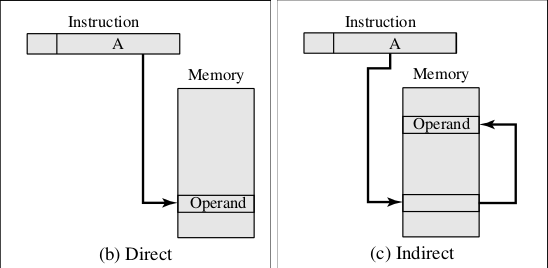
\includegraphics[scale=0.65]{./imagens/enderecamento.png}
 \caption{Endereçamento direto e indireto \cite{stallings}}
\label{enderecamento}
\end{figure}

\subsection{Aninhamento de Subprogramas} 
\label{sub:aninhamento_de_subprogramas}
Linguagens como ALGOL 68, Pascal e Ada permitem aninhamento de subprogramas, assim como linguagens mais recentes como JavaScript, Python e Lua. Linguagens descententes de C não permitem aninhamento. O trecho de código a seguir mostra um exemplo de aninhamento de funções em JavaScript.

\begin{verbatim}
function hipotenusa(a, b) {
   function quadrado(x) {
      return x * x; 
   }
   return Math.sqrt(quadrado(a) + quadrado(b));
}
\end{verbatim}%seção 9.4
%!TEX root = ../artigo.tex
\section{Métodos de Passagem de Parâmetros} % (fold)
\label{sec:metodos_passagem_parametros}
A passagem de parâmetros é uma das formas do subprograma ter acesso aos dados que irá processar. 
Os parâmetros podem ser utilizados para apresentar valores ao subprograma e recuperar seu valor após termino do subprograma. Existem dois tipos de parâmetros, os parâmetros no cabeçalho do subprograma são chamados parâmetros formais e os parâmetros apresentados numa chamada ao subprograma são chamados de parâmetros reais. 


Exemplo de cabeçalho de subprograma.
Exemplo de chamada a um subprograma.


Três modelos semânticos de passagem de parâmetros são descritos na literatura: modo entrada (in mode), modo saída (out mode) e modo entrada/saída (inout mode). Estes modelos definem como os dados são transmitidos entre os parâmetros formais e reais. No modo entrada os parâmetros formais podem receber dados do parâmetro real, no modo saída eles podem transmitir dados para o parâmetro real e no modo entrada/saída podem fazer os dois. Estes três modelos básicos de transmissão de parâmetros são utilizados pelos projetistas de linguagem nas implementações dos métodos de passagem de parâmetros.

\subsection{Passagem por valor}
A passagem por valor é um modelo de implementação para parâmetros de modo entrada, onde o parâmetro formal recebe dados do parâmetro real. Nesse modo, o valor do parâmetro real é utilizado para inicializar o parâmetro formal que atua como uma variável local no subprograma.

A transferência dos dados pode ser feita por cópia dos valores ou pela transmissão de um caminho de acesso (ponteiro ou referência) para o valor do parâmetro real. Na passagem por valor normalmente é utilizado a transferência por cópia, visto que para a transmissão do caminho de acesso seria necessário que o dado estivesse numa célula protegida contra escrita, o que não é uma tarefa simples.

Exemplo: Imagine se o subprograma passe o parâmetro para outro subprograma.

O método de passagem por valor é rápida na vinculação e no tempo de acesso. Se for utilizado transferência por cópia, tem como desvantagem a necessidade de espaço adicional para armazenamento e as operações de transferência podem ser custosas se o parâmetro for grande.


\subsection{Passagem por resultado}
A passagem por resultado segue modelo semântico de passagem de parâmetro modo saída. Neste método nenhum valor é transmitido na chamada do subprograma, o parâmetro formal funciona como variável local e antes que o controle retorne para o chamador, o valor do parâmetro formal é copiado para o parâmetro real.

Assim como no método de passagem por valor, a passagem por resultado compartilha as desvantagens da necessidade de armazenamento e operações extras caso for retornado valores em vez do caminho de acesso. Porém devido a dificuldade de implementação da passagem por resultado transmitindo um caminho de acesso utilizamos a transferência por cópia, dificuldade esta de garantir que o valor inicial do parâmetro real não seja utilizado no subprograma chamado.

Ainda como desvantagem existe o problema colisão de parâmetros reais. Suponha um subprograma com dois parâmetros formais diferentes, na chamada do subprograma atribuicao(a,a) qual será o valor retornado para a? Será retornado o valor que for atribuído por último ao parâmetro real a. Mas essa ordem depende da implementação. Exemplo de colisão de parâmetros reais em C\#:

\begin{verbatim}
void atribuicao(out int x, out int y) {
    x = 29;
    y = 15;
}
...
f.atribuicao(out a, out a);
\end{verbatim}

Outro problema é na escolha do tempo para avaliar os endereços dos parâmetros reais (momento da chamada ou momento do retorno). 

Por exemplo, no subprograma abaixo o resultado pode depender do tempo de avaliação do endereço. Como a variável index pode ser modificada pelo subprograma, o parâmetro formal x pode assumir valores distintos dependendo da ordem de avaliação caso houver uma chamada deste subprograma passando uma lista como parâmetro real.

\begin{verbatim}
void subprograma(out int x, int index) {
    x = 23;
    index = 5;
}
...
sub = 21;
f.subprograma(list[sub], sub);
\end{verbatim}

Se o endereço é avaliado na entrada do subprograma o valor 23 é atribuído a list[21], se for avaliado na saída o valor 23 é atribuído a list[5].


\subsection{Passagem por valor-resultado}
A passagem por valor-resultado é a implementação de parâmetro em modo entrada/saída onde é combinado a passagem por valor e a passagem por resultado. O valor do parâmetro real é usado para inicializar o parâmetro formal que atua como variável local. No termino do subprograma o valor do parâmetro formal é transmitido de volta para o parâmetro real. 

A passagem por valor-resultado também é chamada de passagem por cópia (porque o parâmetro real é copiado para o parâmetro formal na chamada do subprograma e é copiado de volta para o parâmetro real no fim do subprograma) e partilha dos mesmos problemas da passagem por valor e passagem por resultado.

\subsection{Passagem por referência}
Mais um modelo de implementação de parâmetros em modo entrada/saída. O parâmetro real é compartilhado com o subprograma chamado pela transmissão de uma caminho de acesso.
A passagem por referência traz como vantagem o custo de tempo e espaço, pois não é necessário espaço duplicado e nem operações de cópia. Como desvantagem o acesso ao parâmetro formal é mais lento do que a passagem por valor devido ao endereçamento indireto, ou seja, é preciso mais de um acesso para chegar ao valor da variável. Além disso, se for necessário uma comunicação unidirecional torna-se um problema, pois pode haver mudanças no parâmetro real.

Presença de problemas como colisões de parâmetros reais e de apelido. A função em C++ abaixo ilustra o problema de apelido que é prejudicial para legibilidade e confiabilidade do código.

\begin{verbatim}
void função(int &first, int &second)
...
função(total, total)
\end{verbatim}

\subsection{Passagem por nome}
A passagem por nome é mais um método de transmissão de parâmetros em modo entrada/saída. O parâmetro real é textualmente substituído pelo parâmetro formal em todas as suas ocorrências no subprograma. O parâmetro formal é vinculado a valores ou a endereços reais, mas a vinculação real é retardada até o momento que o parâmetro formal seja atribuído ou referenciado.

Esse método é complexo de implementar e ineficiente, porém é usado em tempo de compilação para parâmetros genéricos de subprogramas genéricos em C++, Java 5.0 e C\# 2005.


\subsection{Implementando métodos de passagem de parâmetros}
A comunicação de parâmetros é realizada por uma pilha em tempo de execução que é gerenciada pelo sistema. 

Na passagem de parâmetros por valor são copiados valores dos parâmetros reais para posições na pilha que serve como armazenamento para os parâmetros formais correspondentes. Já na passagem por resultado os valores que serão atribuídos ao parâmetro real fica na pilha até que possam ser recuperados pelo chamador após o término da chamada subprograma. Na passagem por valor-resultado uma posição na pilha é inicializada pela chamada e depois é usado como uma variável local no subprograma chamado. Na passagem por referência apenas é copiado o endereço do parâmetro para a pilha.

Figura.

\subsection{Métodos de passagem de parâmetros das principais linguagens}
O C usa passagem por valor, porém obtêm a semântica da passagem por referência utilizando ponteiros (copiado do ALGOL 68). O valor do ponteiro como parâmetro é copiado para a função chamada e nada é retornado, entretanto a função chamada pode fazer alterações naquele dado uma vez que possui o caminho de acesso. A proteção contra escrita é feita implicitamente na função chamada. 

O C++ utiliza também a passagem por valor e garante a passagem por referência com ponteiros, além de um tipo especial de ponteiro chamado tipo de referência que após sua inicialização não pode referenciar outra variável.

Em Java os parâmetros também são passados por valor, porém como os objetos são apenas acessados por variáveis de referência os parâmetros são passados com a semântica de referência.
Ada e Fortran 95+ permitem ao programador especificar o modo de cada parâmetro formal (entrada, saída e entrada-saída).

O C\# utiliza a passagem por valor como padrão, mas também permite ao programador utilizar passagem por refreferência se o prefixo \textbf{\emph{ref}} for utilizado antes dos dois parâmetros (real e formal). Também suporta passagem de parâmetro em modo saída, passado por referência, com o modificador out antes do parâmetro formal.

A passagem de parâmetro do PHP é semelhante à do C\#, excepto que tanto o parâmetro real quanto parâmetro formal pode ser passado por referência precedendo um ou ambos os parâmetros com uma comercial (\&).

Em Python e Ruby é utilizado a passagem por atribuição, nesse sentido todos os valores de dados são objetos. Assim cada variável armazena uma referencia para o valor. Se uma variável referenciada é acrescida de uma unidade então é criado um novo objeto com o valor da variável mais 1 e a variável referencia o novo objeto. No caso de vetor passado como parâmetro se houver uma atribuição ao parâmetro formal que referencia o vetor então não tem efeito no chamador, porém se houve uma atribuição à um elemento do vetor passado então o correspondente parâmetro real será modificado.

\subsection{Verificação de tipos}
\label{sub:verificacao_de_tipos}
A verificação dos tipos dos parâmetros reais em relação aos seus correspondentes parâmetros formais faz-se necessária uma vez que erros causados por tipos de parâmetros diferentes podem levar a erros de programa difíceis de detectar. Desta forma em muitas linguagens é feita a verificação de tipos.

Nas versões recentes do C e do C++ é feita verificação de tipos, onde os tipos dos parâmetros formais são incluídos na lista no cabeçalho da função. Não existe verificação de tipos de parâmetros em Python e Ruby porque estas linguagens são dinamicamente tipadas.


% section metodos_passagem_parametros (end)


%seção 9.5
%!TEX root = ../artigo.tex

\section{Subprogramas Como Parâmetro} % (fold)
\label{sec:subprogramas_como_parametro}
Em muitas ocasiões temos a necessidade de passar um subprograma através de um parâmetro. A ideia é interessante e simples, mas gera duas complicações em termos de implementação.

Primeiro, temos a complicação que consiste na maneira de realizar a checagem de tipo (\textit{type checking}, ~\ref{ub:verificacao_de_tipos}) do subprograma passado por parâmetro. Em C e C++, onde a passagem de subprogramas é feita através de ponteiro para função, essa checagem é feita pelo tipo do ponteiro.

A outra complicação ocorre em linguagens de programação que permitem subprogramas aninhados. O problema refere-se a qual ambiente de referência o subprograma passado por parâmetro terá. Nessa situação, há três tipos possíveis:
\begin{description}
	\item[Shallow Binding:] O ambiente é o local onde o subprograma é chamado.
	\item[Deep Binding:] O ambiente refere-se onde o subprograma foi definido.
	\item[Ad Hoc Binding:] O ambiente condiz com o local que o subprograma foi passado por parâmetro.
\end{description}

Como exemplo, considere a listagem ~\ref{scope_binding}, cuja sintax é de JavaScript. O subprograma \textit{sub2()} apenas imprime o valor da variável \textit{x}, porém, seu valor depende do ambiente de referência utilizado. 

\begin{lstlisting}[caption=Código retirado de \cite{sebesta}]
function sub1() {
	var x;
	function sub2() {
		alert(x);
	};
	function sub3() {
		var x;
		x = 3;
		sub4(sub2);
	};
	function sub4(subx) {
		var x;
		x = 4;
		subx();
	};
	x = 1;
	sub3();
};
\end{lstlisting}
\label{scope_binding}

Caso a listagem em questão utilize o ambiente de referência \textit{Shallow Binding}, o valor impresso seria 4. Caso o ambiente \textit{Deep Binding} fosse escolhido, o valor impresso seria 1. Já para \textit{Ad Hoc Binding}, o valor seria 3.

Segundo Robert W. Sebesta, a abordagem \textit{Ad Hoc Binding} nunca foi implementada \cite{sebesta}.
% section subprogramas_como_parametro (end)%seção 9.6
%!TEX root = ../artigo.tex
\section{Chamar Subprogramas Indiretamente} % (fold)
\label{sec:chamar_subprogramas_indiretamente}
Há momentos, durante a programação de um software, em que se torna necessário chamar subprogramas de forma indireta. Isso ocorre quando o subprograma a ser chamado é somente conhecido em tempo de execução, como eventos disparados por bibliotecas de interface gráfica e funções de \textit{callback}.

%exemplo em c/c++
Em C e C++, podemos utilizar ponteiro para função para chamar um subprograma conhecido em tempo de execução \cite{pointer,sebesta}. Para utilizar essa técnica, primeiro temos que declarar uma função, como por exemplo:
\begin{verbatim}
int sum(int a, int b)
{
    return a + b;
}
\end{verbatim}

A seguir, temos que declarar um ponteiro com a mesma assinatura da função escolhida. Como no nosso exemplo (função \textit{sum}) a função possui dois parâmetros e um retorno do tipo \emph{int}, temos um ponteiro como mostrado:
\begin{verbatim}
int (*sum_pointer)(int, int);
\end{verbatim}

Em seguida, é necessário atribuir a função em questão para o ponteiro declarado. Em nosso exemplo:
\begin{verbatim}
sum_pointer = &sum;
\end{verbatim}

Por fim, basta invocar a função, como da seguinte maneira:
\begin{verbatim}
(*sum_pointer)(1,2);	
\end{verbatim}

%exemplo em C#
Em C\#, podemos referenciar métodos em forma de objetos, através do uso de \emph{delegate} \cite{delegate,sebesta}, o que torna muito poderoso e flexível. Para fazer uso do mesmo, precisamos declarar um \emph{delegate} para um determinado protocolo de função, como:
\begin{verbatim}
public delegate int SumDelegate(int a, int b);
\end{verbatim}

Podemos instanciar um SumDelegate passando por parâmetro para seu construtor o nome de uma função cuja declaração tenha o mesmo protocolo. Suponha a existência da função chamada \textit{sum} que respeite essa assinatura, podemos então instanciar SumDelegate como segue:
\begin{verbatim}
SumDelegate sumDelegate= new SumDelegate(sum);
\end{verbatim}

Para executar o \textit{delegate} em questão, fazemos da seguinte forma:
\begin{verbatim}
sumDelegate(2,3);
\end{verbatim}
% section chamar_subprogramas_indiretamente (end)%seção 9.7
%!TEX root = ../artigo.tex
\section{Sobrecarga de Subprogramas} % (fold)
\label{sec:sobrecarga_de_subprogramas}
A maioria das linguagens de progamação permitem sobrecarga de subprogramas, que consiste em subprogramas com o mesmo nome, mas com parâmetros diferentes, seja por quantidade, ordem ou tipo.

Essa técnica é utilizada quando temos subprogramas que tem o mesmo objetivo, porém fazem uso de parâmetros diferentes. Em C++, C\# e Java a sobrecarga de construtores é a mais utilizada por desenvolvedores.

Conforme apontado por Sebesta, as linguagens Ada, Java, C++, C\# e F\# são exemplo de linguagens que permitem sobrecarga de operadores \cite{sebesta}.
% section sobrecarga_de_subprogramas (end)%seção 9.8
%!TEX root = ../artigo.tex
\section{Subprogramas Genéricos} % (fold)
\label{sec:subprogramas_genericos}
No desenvolvimente de software, o reuso do código fonte é um fator importante para aumentar a produtividade e diminuir gastos. Uma maneira de conseguir esse reuso seria fazer um único subprograma funcionar para qualquer tipo de dados. Com isso, por exemplo, não precisamos criar um subprograma de ordenação para cada tipo de dado existente.

Um subprograma polimórfico é algo que pode nos oferecer esse tipo de reuso. Segundo Sebesta \cite{sebesta}, há três tipos de polimorfismo, sendo eles:
\begin{description}
	\item[Ad Hoc:] Consiste na sobrecarga de subprogramas, conforme mostrado na seção \ref{sec:sobrecarga_de_subprogramas}.
	\item[Subtipo:] Específico para linguagens orientadas a objeto, que não está dentro do escopo deste trabalho, mas pode ser encontrado em \cite{poli_java}.
	\item[Paramétrico:] Baseia-se do uso de tipos genéricos, onde esse tipo genérico pode assumir qualquer tipo de dado. Esta seção irá abordar esse tipo de polimorfismo.
\end{description}

Subprogramas com polimorfismo paramétrico são subprogramas que utilizam tipos de dados genéricos, o que possibilita seu reuso para cada tipo de dado. A seguir, iremos exemplificar o uso dessa técnica em C++, Java e C\#.

%-------------Templates em C++
\subsection{Template em C++} % (fold)
\label{sub:template_em_c}
Em C++, funções genéricas são obtidas através do uso de \emph{templates} \cite{template_cpluplus}. Primeiro, é necessário declarar um template, fazendo-o da seguinte forma:
\begin{verbatim}
template <template parameters>
\end{verbatim}

Um \emph{template parameter} pode ter uma das seguintes formas
\begin{verbatim}
class identifier
typename identifier
\end{verbatim}

Segundo Sebesta \cite{sebesta}, a palavra chave \emph{class} é utilizada para especificar tipos e \emph{typename} é necessária para especificar um valor absoluto.

Como exemplo, vamos declarar um função template, que retorna o maior valor entre dois dados. A declaração é feita da seguinte forma
\begin{verbatim}
template <class myType>
myType GetMax (myType a, myType b) {
   return (a>b?a:b);
}
\end{verbatim}

Para chamarmos \emph{GetMax} para dois inteiros, fazemos da seguinte maneira
\begin{verbatim}
GetMax<int> (1,2);
\end{verbatim}

Para trocar o tipo dos parâmetros da função \emph{GetMax}, basta trocar o tipo de dados ao charmar a função em questão (por exemplo, de \emph{int} para \emph{float}).

\emph{Templates} podem ser utilizado em classes, podem ser aninhados e também podem possuir especializações. Explicar essas funcionalidades não faz parte do escopo deste trabalho, mas isso pode ser obtido em \cite{template_cpluplus}.
% subsection template_em_c (end)

%-------------Métodos Genéricos em Java
\subsection{Métodos Genéricos em Java} % (fold)
\label{sub:metodos_genericos_em_java}
Em Java, podemos fazer o uso de métodos genéricos, sendo similar aos \emph{templates} de C++. Um exemplo de um método genérico em Java é como segue
\begin{verbatim}
public static <T> T doIt(T[] list) {
   ...
}
\end{verbatim}

Onde é definido o método \emph{doIt} que recebe como parâmetro uma lista de tipos genéricos. O método \emph{doIt} pode ser chamado passando uma lista do tipo \emph{String} da seguinte forma
\begin{verbatim}
	doIt<String>(myList);
\end{verbatim}

Diferentemente de C++, os tipos genéricos em java devem ser uma classe, não podendo ser um valor absoluto ou um tipo primitivo. Além do mais, Java permite que limitamos os tipos genéricos, como informando de qual classe ele deve herdar ou qual interface deve implementar \cite{sebesta}.

Tipos genéricos em Java nos fornece muitos outros recursos (como \emph{Wildcards}), que não abordados neste trabalho, mas que podem ser encontrados com detalhes em \cite{generics_java}.
% subsection metodos_genericos_em_java (end)

%-------------Métodos Genéricos em C#
\subsection{Métodos Genéricos em C\#} % (fold)
\label{sub:metodos_genericos_em_c_sharp}
Métodos genéricos em C\# tem as mesmas funcionalidades de Java, porém não suportam \emph{wildcards}. Uma diferença em C\# é que o tipo do argumento pode ser omitido caso o compilador poder inferir o tipo \cite{sebesta}. 

Mais informações e exemplos sobre tipos genéricos em C\# podem ser encontrados em \cite{generics_msdn}.
% subsection metodos_genericos_em_c_sharp (end)

% section subprogramas_genericos (end)

%seção 9.9
\section{Questões de projetos referente a funções} 
\label{sec:questoes_de_projetos_referentes_a_funcoes}
Algumas questões relevantes ao projeto em relação a funções precisam ser levados em conta. As próximas seções discutem sobre questões de efeitos colaterais, tipos de retorno e quantidade de valores de retorno.

\subsection{Efeitos colaterais}
\label{sub:efeitos_colaterais}
Uma questão relevante ao projeto em relação a funções é se efeitos colaterais serão permitidos. Linguagens puramente funcionais como Haskell, não possuem variáveis e portanto suas funções não possuem efeitos colaterais. Já linguagens que permitem funções com parâmetros passados por valor ou por referência, possuem efeitos colaterias, como por exemplo \textit{aliasing} (\textit{alias}, apelido). Considere o exemplo a seguir.

\begin{verbatim}
int x = 3; 
... // se int* y = &x;
*y = 9;
\end{verbatim}

O compilador nada pode fazer para otimizar o código acima, uma vez que não é possível saber se y = \&x. Então, se o otimizador tentar aplicar, por exemplo, o constant propagation sabendo que x é 5, e y for um \textit{alias}, ponteiro para x, então a propagação será feita de forma errada. 

\subsection{Tipos de Valores Retornados}
\label{sub:tipos_de_valores_retornados}
C permite qualquer tipo ser retornado por suas funções exceto vetores e funções. Ambos nesse caso podem ser manipulados por ponteiros. C++ é semelhante ao C mas também permite tipos definidos pelo usuário ou classes serem retornados. Fortran 77 e Pascal permitem apenas tipos não estruturados. Ada, Python, Ruby e Lua, retornam valores de qualquer tipo, exceto no caso do Ada, onde funções não são tipos, portanto não podem ser retornadas (mas ponteiros para funções sim). Em Java e C\#, qualquer tipo ou classe podem ser retornados por seus métodos, porém, como método não é um tipo, não pode ser retornado.

\subsection{Quantidade de valores retornados}
\label{sub:quantidade_de_valores_retornados}
A maioria das linguagens atuais permitem apenas 1 valor de retorno. A linguagem Lua, permite o retorno de multiplos valores. Considere um exemplo de função na linguagem Lua que retorna 3 valores \cite{sebesta}. A ordem das variáveis que chamam a função, serão vinculadas na ordem dos valores retornados pela função. \\

\noindent A chamada da função

\begin{verbatim}
a, b, c = fun() 
\end{verbatim}
Onde o retorno da função fun() é 
\begin{verbatim}
return 3, sum, index
\end{verbatim}

%seção 9.10
\section{Sobrecarga de operadores definidos pelo usuário}
\label{sec:sobrecarga_operadores_definidos_pelo_usuario}
Linguagens como Ada, Python, Ruby e C++ suportam sobrecarga de operadores (\textit{Overloaded Operators}). Sobrecarga de operadores permite efetuar operações como soma, subtração, multiplicação e divisão em tipos de dados definidos pelo usuário. Considere a listagem \ref{lst:overload_c}, que realiza a sobrecarga do operador + para efetuar a soma de vetores. A saída do programa é 4, 3.

\begin{lstlisting}[caption={Código retirado de \cite{overload_c}}, label={lst:overload_c}]
#include <iostream>

using namespace std;

class CVector {
  public:
    int x,y;
    CVector () {};
    CVector (int,int);
    CVector operator + (CVector);
};

CVector::CVector (int a, int b) {
  x = a;
  y = b;
}

CVector CVector::operator+ (CVector param) {
  CVector temp;
  temp.x = x + param.x;
  temp.y = y + param.y;
  return (temp);
}

int main () {
  CVector a (3,1);
  CVector b (1,2);
  CVector c;
  c = a + b;
  cout << c.x << "," << c.y;
  return 0;
}
\end{lstlisting}%seção 9.11
\section{Closure}
\label{sec:closure}
Closure é uma variável local em uma função que é mantida viva (não é desalocada) após o retorno dessa função. Apenas linguagens que permitem subprogramas aninhados é possivel closure. Linguagens como C\# e JavaScript possuem closure. Considere a listagem \ref{lst:closure}, na linguagem JavaScript, que utiliza closure.

\begin{lstlisting}[caption={Closure em JavaScript}, label={lst:closure}]
function foo(x) {
  var tmp = 3;
  return function (y) {
    alert(x + y + (++tmp));
  }
}

var bar = foo(2);
bar(10); 
\end{lstlisting}

\noindent
No programa acima na linha 8, bar é um closure. A saída do programa exibe 16 como saída quando executado pela primeira vez, e vai incrementando em 1 a cada execução.%seção 9.12
\section{Co-rotinas} 
\label{sec:co_rotinas}
Co-rotinas são um tipo especial de subprogramas. A linguagem Lua é uma das linguagens que possui co-rotinas. Co-rotinas possuem múltiplos pontos de entrada controlados elas mesmas. A cada execução (chamado de resumo), a co-rotina volta a sua execução não do início, mas sim de algum outro ponto (por isso resumo). Co-rotinas mantém seu estado entre as ativações e portanto são sensíveis ao histórico, ou seja, possuem variáveis estáticas.

Geralmente, corrotinas são criadas pela aplicação por uma unidade chamada de unidade mestre. A unidade mestre não é uma co-rotina, é tem a função de ativar uma das co-rotinas, que após suas inicializações, resumem uma as outras até que a execução de todas termine e o controle volte para a unidade mestre. As figuras \ref{co-rotinas} e \ref{co-rotinas_b} ilustram o possível funcionamento de duas co-rotinas A e B.

\begin{figure}[ht!]
 \centering
 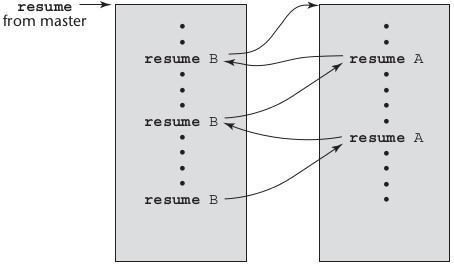
\includegraphics[scale=0.65]{./imagens/coroutines.png}
 \caption{Execução de co-rotinas 1 \cite{sebesta}}
\label{co-rotinas}
\end{figure}

\begin{figure}[ht!]
 \centering
 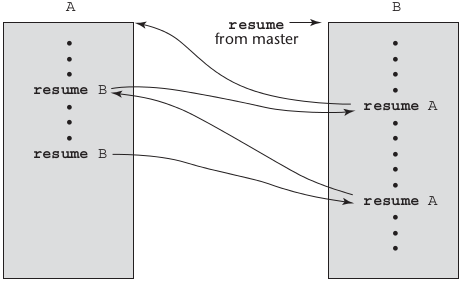
\includegraphics[scale=0.65]{./imagens/coroutines_b.png}
 \caption{Execução de co-rotinas 2 \cite{sebesta}}
\label{co-rotinas_b}
\end{figure}
%seção 9.13

\bibliographystyle{plain} % especifica o estilo como as refer?ncias s?o formatadas
\bibliography{artigo} % especifica o arquivo que cont?m todas as refer?ncias catalogadas, de acordo com a sintaxe de um arquivo .bib.
\end{document}